
%%%%%%%%%%%%%%%%%%%%%%%%%%%%%%%%%%%%%%%%%%%%%%%%%%%%%%%%%%%%%%%%%%%%
%%%%%%%%%%%%%%%%%%%%%%%%%%%%%%%%%%%%%%%%%%%%%%%%%%%%%%%%%%%%%%%%%%%%
\chapter{WebObs metadata database interface} \label{metadata}



% ==================================================================
\section{Theia$\vert$OZCAR Information System} \label{theia}

Theia$\vert$OZCAR is an Information System which aims to collect the data from different observatories that have different data management methods. Some observatories working with WebObs needed functionalities to do so. Thus, an interface has been made between WebObs and the Theia$\vert$OZCAR IS. This data flux is based on the \textit{FAIR} data principles which stands for:

\begin{itemize}
\item 	 F : easy (\textit{facile} in french) to find;
\item 	 A : accessible;
\item 	 I : interoperable;
\item 	 R : reusable.
\end{itemize}

It is expected in the future that this bridge created between WebObs and the Theia$\vert$OZCAR IS can be reused between WebObs and others data portal. That is why the principle of the Theia$\vert$OZCAR pivot model is presented here but it will be a more general pivot model in the future.

% ==================================================================
\section{Theia$\vert$OZCAR pivot model}

In order to exchange information between WebObs and the Theia$\vert$OZCAR IS, some functionalities have been created to transfer necessary metadata for the Theia$\vert$OZCAR gateway. Those functionalities have been inspired by the Theia$\vert$OZCAR pivot model, based on the ISO19115$/$INSPIRE, O$\&$M and DataCite standards. This model contains the metadata which describes the \textbf{data producer}, the \textbf{datasets} that the \textbf{producer} provides and the \textbf{observations} contained in each of the \textbf{dataset}. An \textbf{observation} describes an \textbf{observed property} (a row in the calibration file) at a given {station} (a \wo{node}) following a \textbf{procedure} and its \textbf{results} (the raw data). 

Note that the metadata database is decoupled from the WebObs configuration file in a manner such as if the Theia required metadata are erased from the metadata database, the genuine related \wo{node}s are not erased from WebObs. On the contrary, erasing a \wo{node} means erasing the related dataset and affiliated metadata. Finally, the deletion of a producer will delete all the datasets (and thus the observations) related to the producer without erasing the NODEs and related calibration files, raw data, etc.

% ==================================================================
\subsection{Metadata structure}

Those informations are gathered by WebObs in a JSON file which respects the structure above (or see the figure below). 3 levels of importance exist for filling informations : mandatory (M), recommended (R) and optionnal (O).

\begin{figure}[!h]
	\centering
	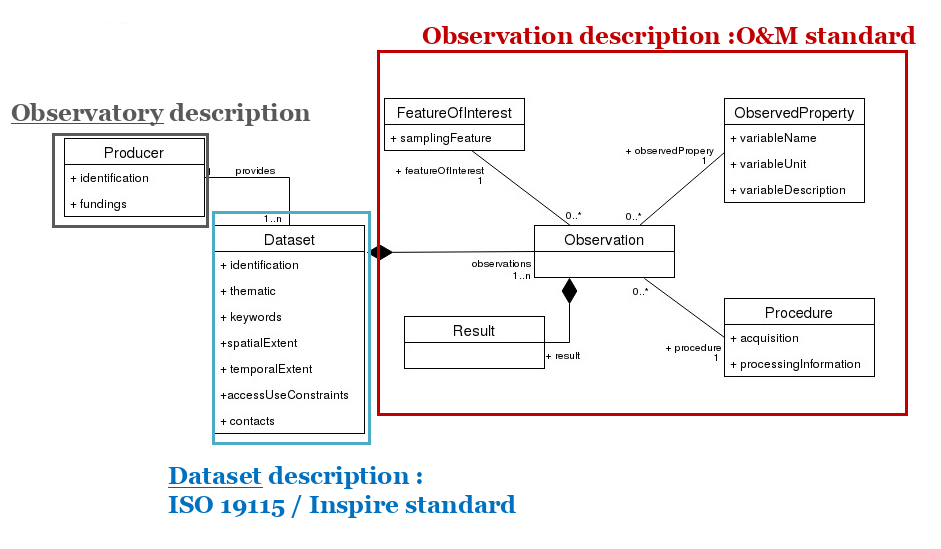
\includegraphics[width=\textwidth]{figures/theia/pivot_model.png}
	\caption{Figure from \url{https://github.com/theia-ozcar-is/csv-to-theia-ozcar-pivot-model}.}
	\label{pivot_model}
\end{figure}

At the highest in the hierarchy are 3 JSON objects :

\begin{itemize}
\item 	 producer;
\item 	 datasets;
\item 	 version.
\end{itemize}

datasets is a collection of dataset JSON object. Each dataset contains 3 informations :

\begin{itemize}
\item 	 identifier;
\item 	 metadata;
\item 	 observations
\end{itemize}

observations is a collection of observation JSON object. producer, dataset and observation parameters are detailed in the sections below.

% ==================================================================
\subsubsection{Producer metadata}

The producer metadata are : 

\begin{itemize}
\item 	 Identifier (M) : identifier for the observtories concerned by the Theia$\vert$OZCAR IS have already been provided to the concerned laboratories;
\item 	 Name (M) : name of the observatory;
\item 	 Title (M) : title of the data producer;
\item 	 Description (M) : a description of the data producer;
\item 	 Objective (R) : a summary of the scientific objectives of the data producer;
\item 	 Measured variables (R) : a summary of the variables observed by the data producer;
\item 	 Email (M) : generic email to contact the data producer;
\item 	 Contacts (M) : first names, last names, emails and roles of the data producer. 2 roles exist: Project leader and Data manager. The project leader is the scientific manager of the observatory, the Data manager is the person in charge of the data management;
\item 	 Funders (M) : types of organisations, scanR identifiers and names of the organisations that fund the data producer;
\item 	 Online resource (O) : link towards the website of the data producer, links to download data, doi and webservice. For the moment, the webservice type is not working.
\end{itemize}

% ==================================================================
\subsubsection{Dataset metadata}

The dataset metadata are : 

\begin{itemize}
\item 	 Identifier (M) : each dataset identifier is based on the data producer identifier as following : $PRODUCERID\_DAT\_DATASETID$;
\item 	 Title (M) : title of the dataset;
\item 	 Description (M) : summary of the dataset, such as definition of the measured variables, the purpose of the study or the geographic location;
\item 	 Subject (M) : lists of keywords and INSPIRE theme;
\item 	 Creator (M) : lists of contacts for the dataset (people in charge of the dataset). Same informations registered as in producer.contacts. 2 roles exist : Publisher and Principal investigator. A Publisher is the person in charge of the data management, the Principal investigator is the scientific referent of the dataset. At least one Principal investigator is required;
\item 	 Spatial coverage (M) : wkt object referencing the spatial extent of the dataset in latitude/longitude;
\item 	 Lineage (M) : describes the life cycle of the dataset, from the acquisition to the data entry via the data treatment.
\end{itemize}

% ==================================================================
\subsubsection{Observation metadata}

The observation metadata are : 

\begin{itemize}
\item 	 Identifier (M) : each dataset identifier is based on the data producer identifier as following : $PRODUCERID\_OBS\_DATASETID$;
\item 	 Processing level (O) : Raw data, Quality-controlled data, Derived products;
\item 	 Data type (M) : Numeric, Text, Vector, Raster, Photo, Video, Audio, Other;
\item 	 Temporal extent (M) : startDate/endDate, format ISO 8601 "YYYY-MM-DDThh:mm:ssZ";
\item 	 Observed property (M) : name of the variable of the observed phenomenon;
\item 	 Station name (M) : name of the acquisition station;
\item 	 Dataset (M) : identifier of the dataset whom the observation belongs to;
\item 	 Data file name (M) : name of the file containing the observations (.csv, .txt, .dat, etc.).
\end{itemize}

For a complete description, please refer to the official documentation of the \href{https://theia-ozcar.gricad-pages.univ-grenoble-alpes.fr/doc-producer/producer-documentation.html#modele-de-donnees-pivot}{Theia$\vert$OZCAR pivot model}.

% ==================================================================
\subsection{Filling the metadata file}
First of all, one has to make sure (only user with administrator right) WEBOBS.rc is rightly configurated like it is shown below \ref{webobs.rc}, in order to display anything Theia$\vert$OZCAR related and to make sure the file theia.rc will be filled. This last configuration file is important because it gathers the metadata the users want to send to Theia$\vert$OZCAR data portal. ROOT\_OUTE is the path name where the data will be saved. For each upload, a sub directory will be created with a zip archive containing the metadata file in JSON format and zip archives with the data files. PASSWORD\_THEIA is the password you have to ask to the Theia$\vert$OZCAR team to upload data.

\begin{figure}[!h]
	\centering
	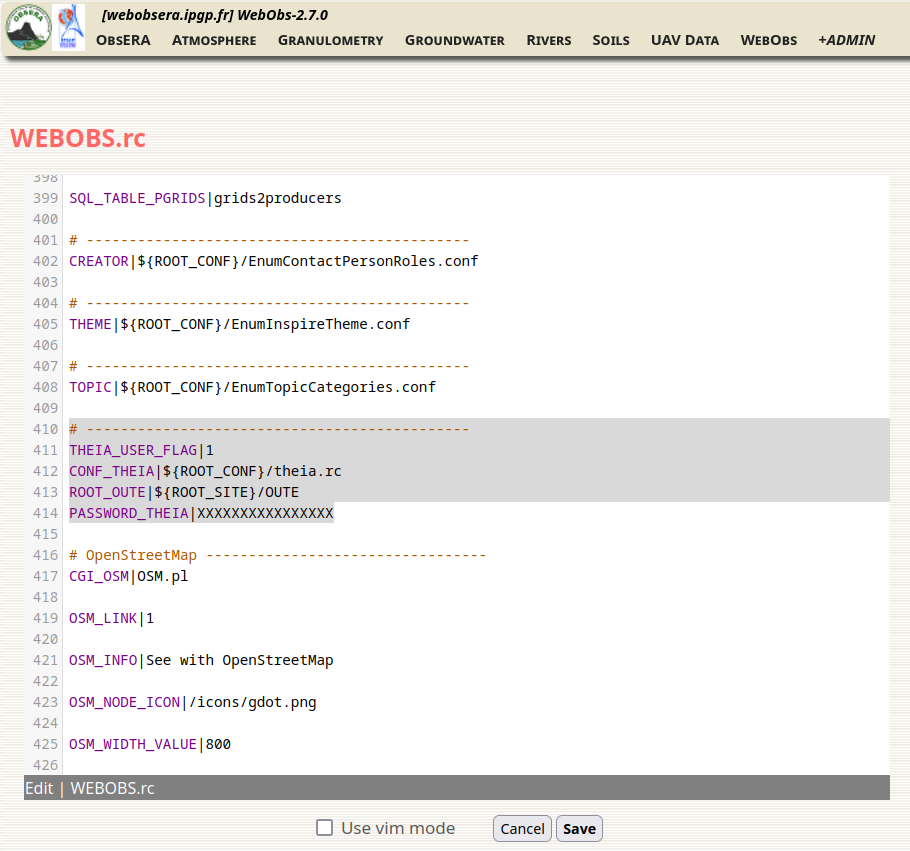
\includegraphics[width=\textwidth]{figures/theia/webobs.rc.png}
	\caption{$THIEA\_USER\_FLAG$ must be 1 to display the metadata resume board and anything metadata related.}
	\label{webobs.rc}
\end{figure}

Each of the three main objects of the pivot model (producer, datasets, observations) can be filled through WebObs, and some are even done automatically, for example when creating a \wo{node}, or when filling the THEIA category. When this has been configured \ref{menu_config}, a link \ref{showTHEIA} to a summary table displaying the metadata is available \ref{recap_table}. To do so, an user with administrator right has to create a link towards the showTHEIA.pl script through +ADMIN $\rightarrow$ Admin editors $\rightarrow$ MAIN MENU EDIT.

\begin{figure}[!h]
	\centering
	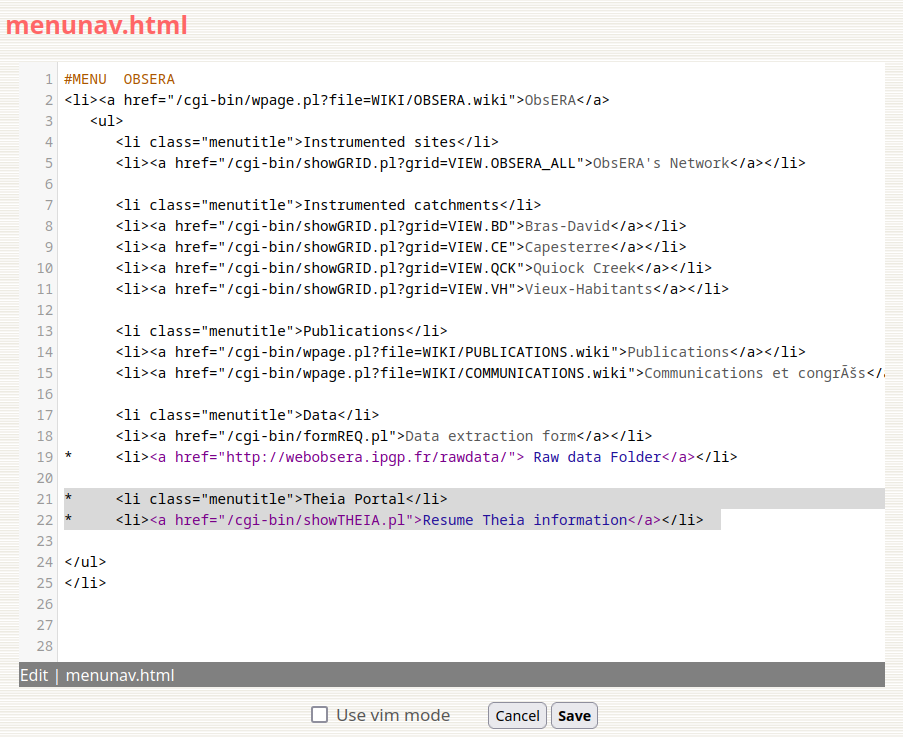
\includegraphics[width=\textwidth]{figures/theia/menu_config.png}
	\caption{An editor allows you to add a personalized tab for the Theia board}
	\label{menu_config}
\end{figure}

\begin{figure}[!h]
	\centering
	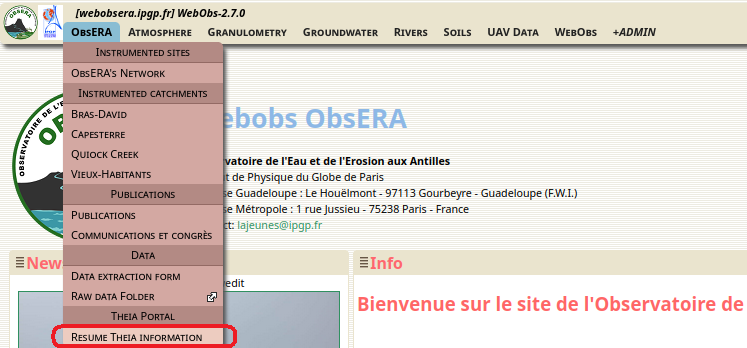
\includegraphics[width=\textwidth]{figures/theia/theia_menu.png}
	\caption{Click on the tab to open the metadata summary table.}
	\label{showTHEIA}
\end{figure}

\begin{figure}[!h]
	\centering
	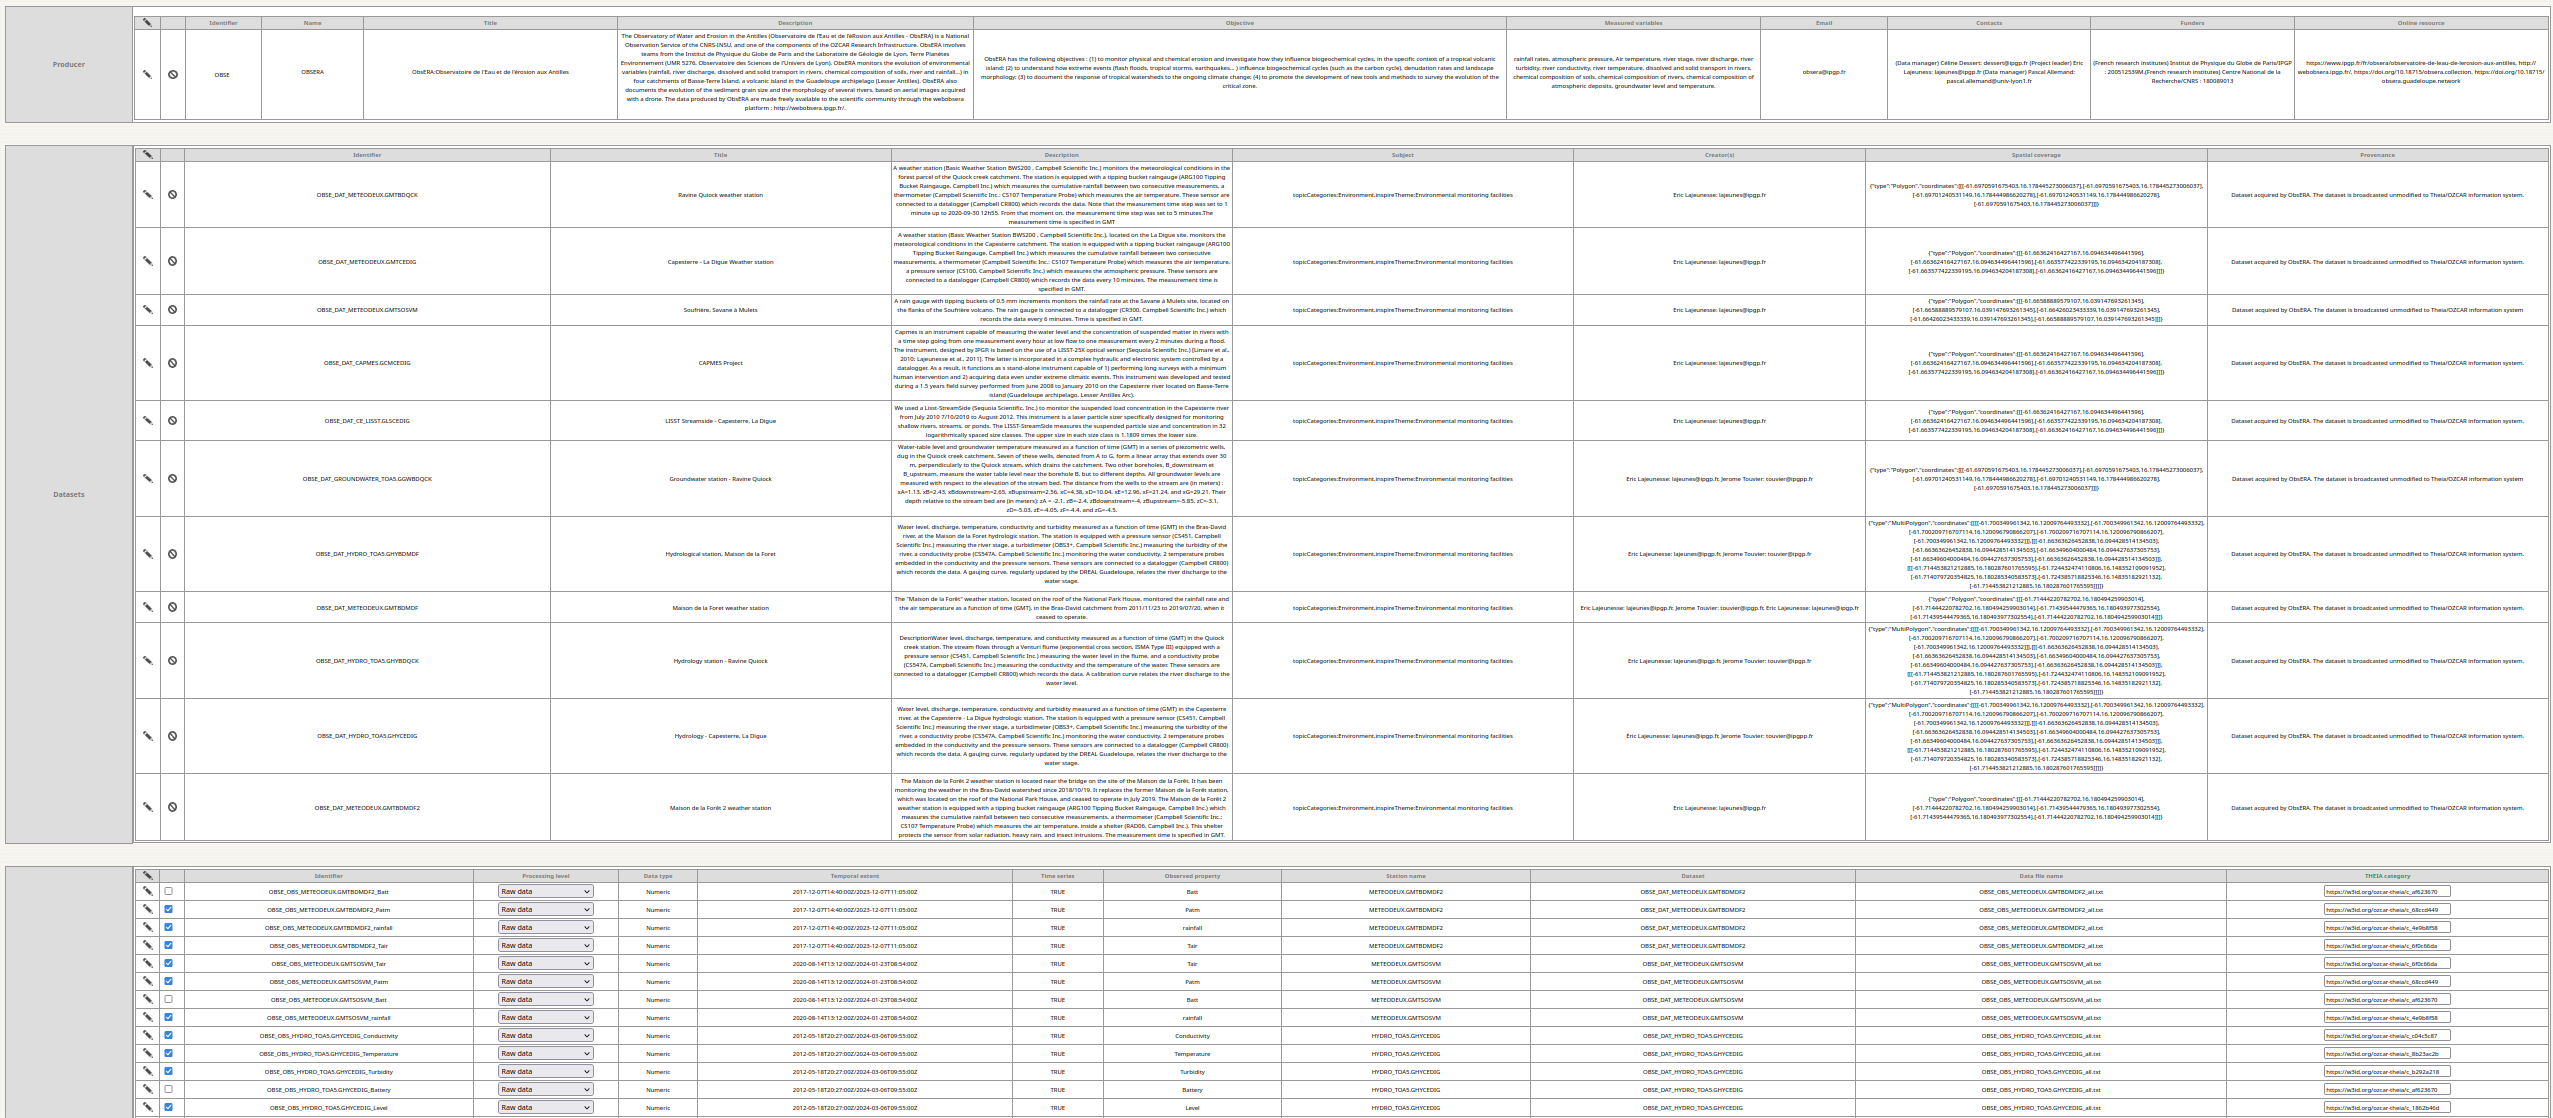
\includegraphics[width=\textwidth]{figures/theia/recap_table.png}
	\caption{The table sums up the mandatory metadata that have been filled to create the JSON file that will be send to the Theia$\vert$OZCAR IS.}
	\label{recap_table}
\end{figure}

By clicking on each row on the pencil, you can get back to the edition menu of the clicked object. If you click on the delete symbol, the row will be deleted from the resume board but not from the database (which will happens when deleting a NODE or a variable in a given .clb file). Moreover, only the rows selected on the resume board will be integrated in the JSON file. Concerning the Theia topic categories, an hyperlink is provided towards the Theia$\vert$OZCAR Skosmos thesaurus. Then, to validate the data you want to send in the JSON file, you have to validate the form. If all the required metadata are validated, a message will appear to confirm the edition of the file called \wo{theia.rc} \ref{theia.rc}.

\begin{figure}[!h]
	\centering
	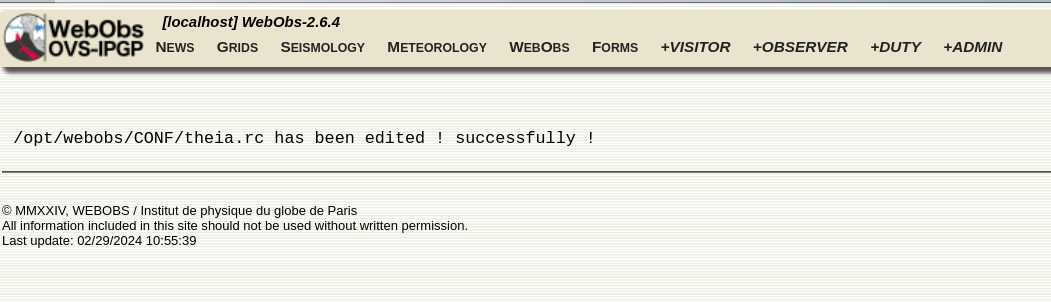
\includegraphics[scale=0.25]{figures/theia/theia_rc.png}
	\caption{If it succeed, a configuration file containing all the information will be edited.}
	\label{theia.rc}
\end{figure}

When launching the job, a .zip file is created for each dataset, containing the observations in a .txt file. Finally, a .zip file is made with the JSON and the datasets .zip files by creating a job using \wo{sendTHEIA.pl} script \ref{sendTHEIA}.

\begin{figure}[!h]
	\centering
	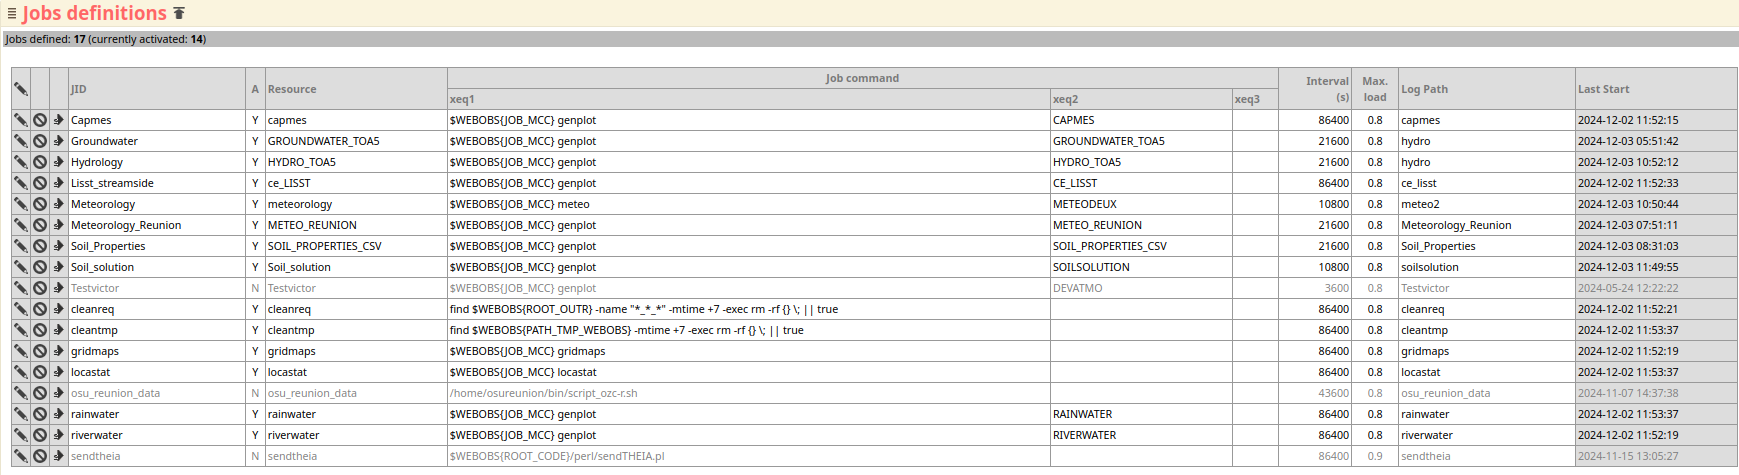
\includegraphics[scale=0.25]{figures/theia/sendTHEIA.png}
	\caption{If it succeed, a .zip file will be downloaded in the OUTE/theia/ directory, containing all the metadata and data ready to send to THEIA pivot model.}
	\label{sendTHEIA}
\end{figure}

% ==================================================================
\subsubsection{Producer metadata}

The producer metadata can be filled throughout the \wo{domain} edition menu \ref{gridsMgr}.

\begin{figure}[!h]
	\centering
	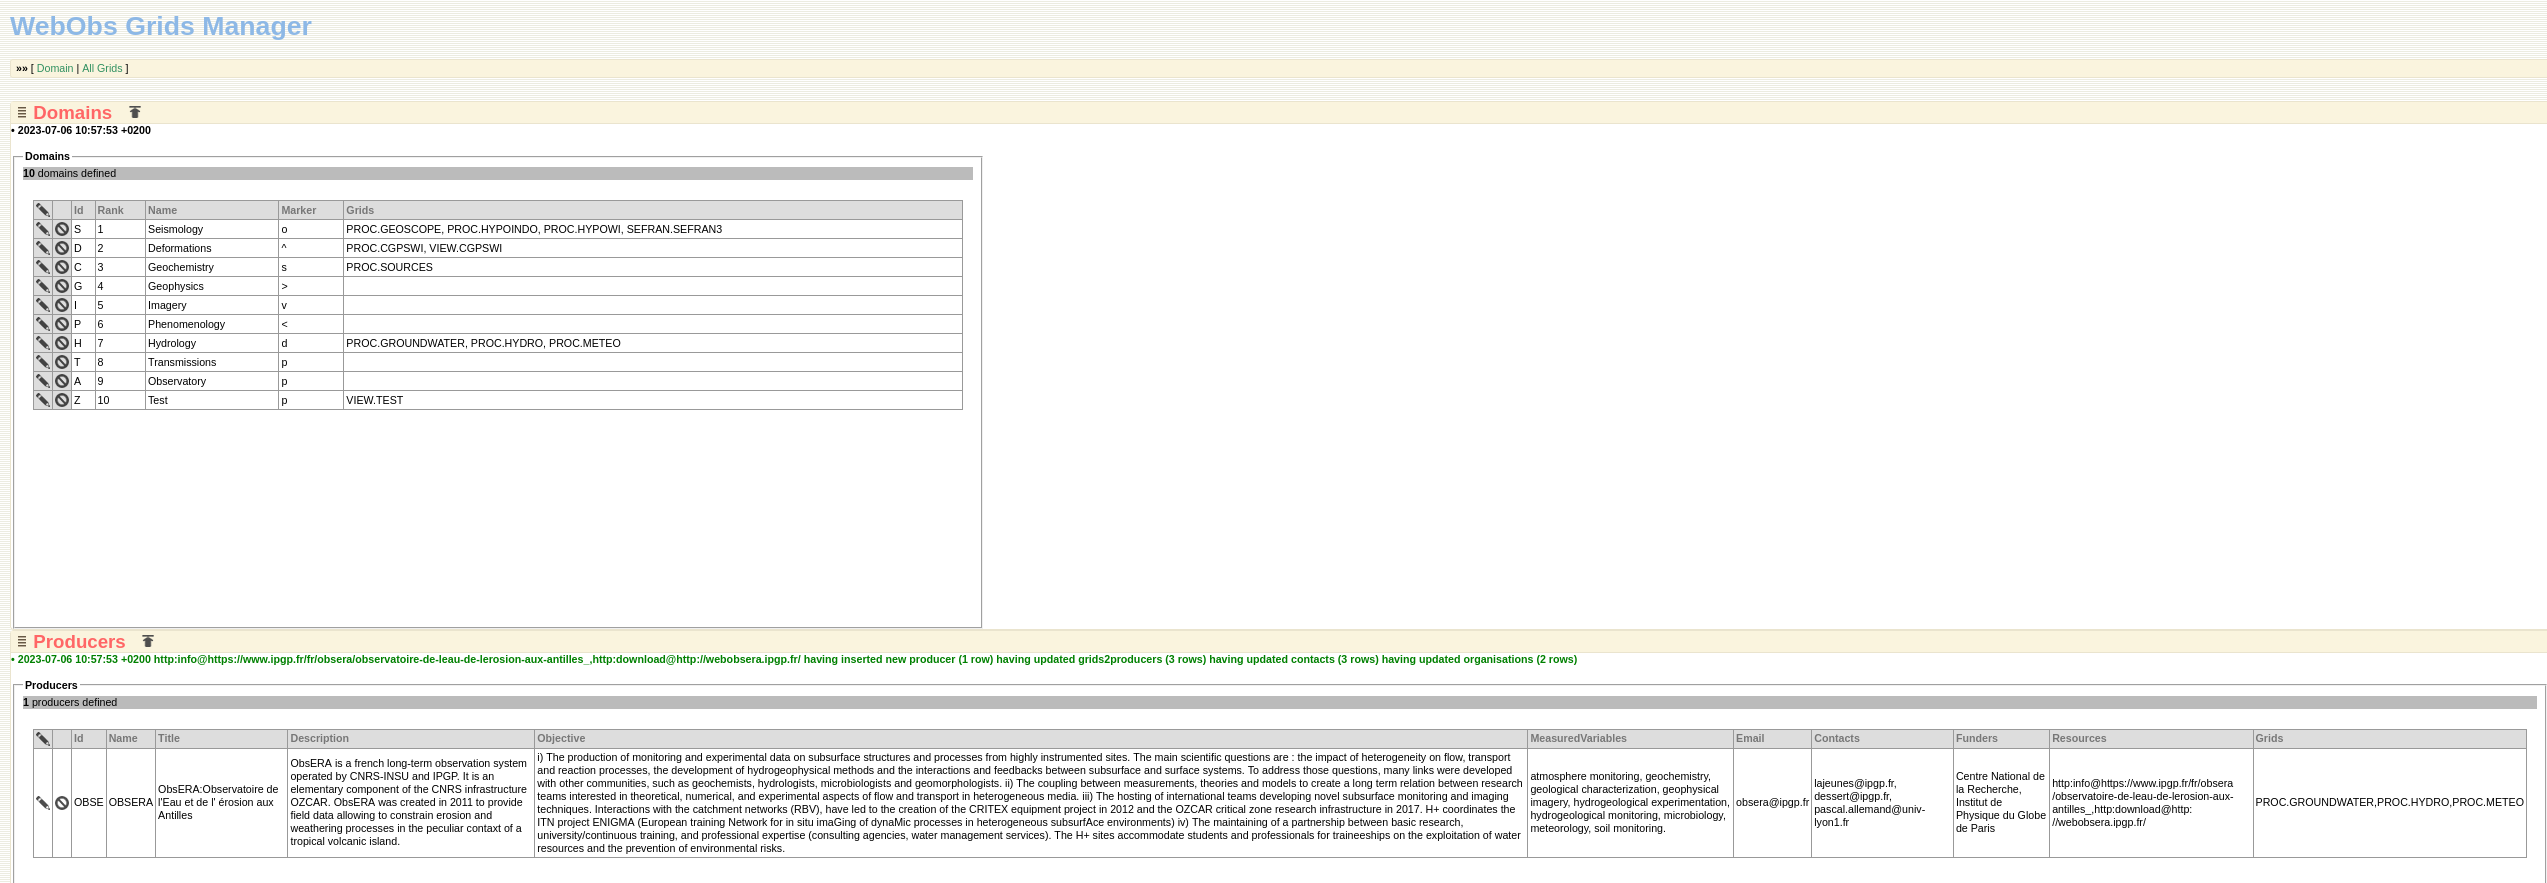
\includegraphics[width=\textwidth]{figures/theia/gridsMgr.png}
	\caption{The table sums up the information about the data producer.}
	\label{gridsMgr}
\end{figure}

Each data producer can be edited or deleted. When creating, deleting or editing a producer, a local SQLite database is filled, called WEBOBSMETA.db, which is only available for the admin. Only the mandatory metadata are necessary, in addition to the grids related to the producer (as several producer can co-exist on the same WebObs).Other metadata are optional even if some are more or less recommended.

% ==================================================================
\subsubsection{Dataset metadata}

Dataset metadata is entered when creating or editing an existing \wo{node} \ref{formNODE}. The \textbf{Name} WebObs \wo{node} fields correspond to the \textbf{dataset.Title} Theia$\vert$OZCAR IS field.

\begin{figure}[!h]
	\centering
	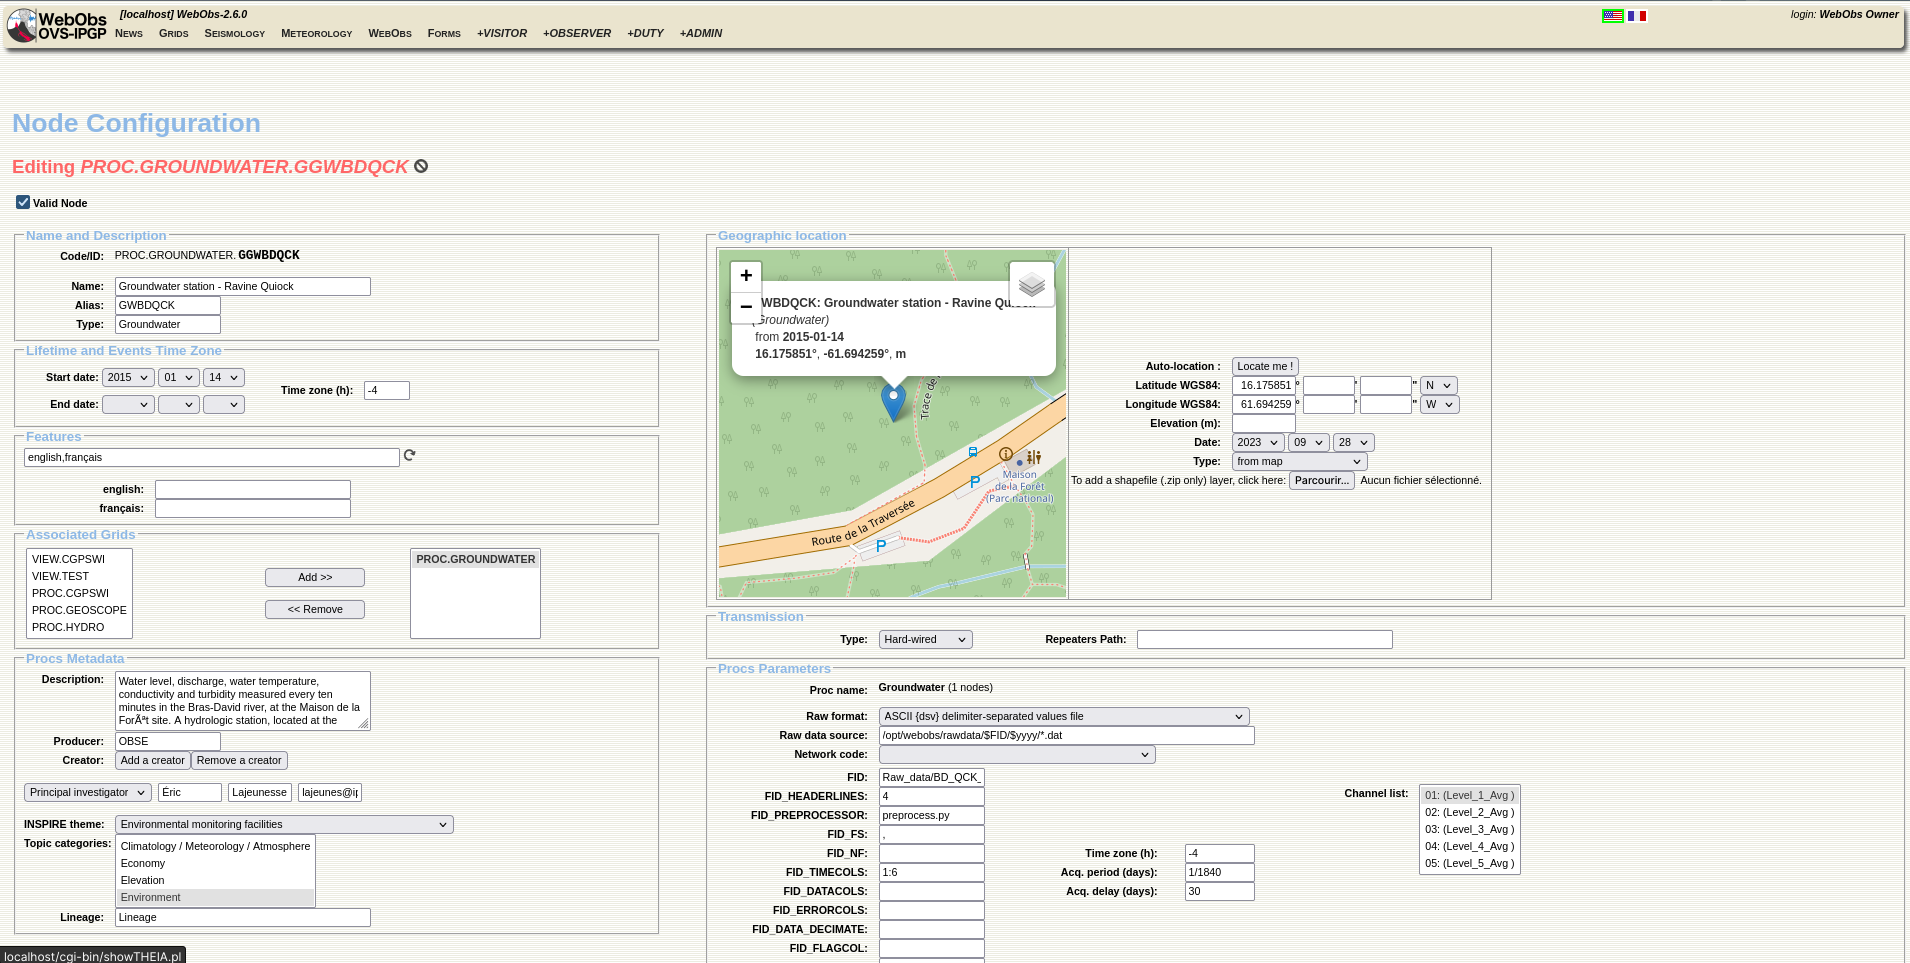
\includegraphics[width=\textwidth, scale=0.4]{figures/theia/formNODE.png}
	\caption{When creating or editing a NODE, fields appear in the left lower panel to fill required metadata in.}
	\label{formNODE}
\end{figure}

% ==================================================================
\subsubsection{Observation metadata}

Observation metadata is entered when creating or editing an existing calibration file \ref{formCLB}.

\begin{figure}[!h]
	\centering
	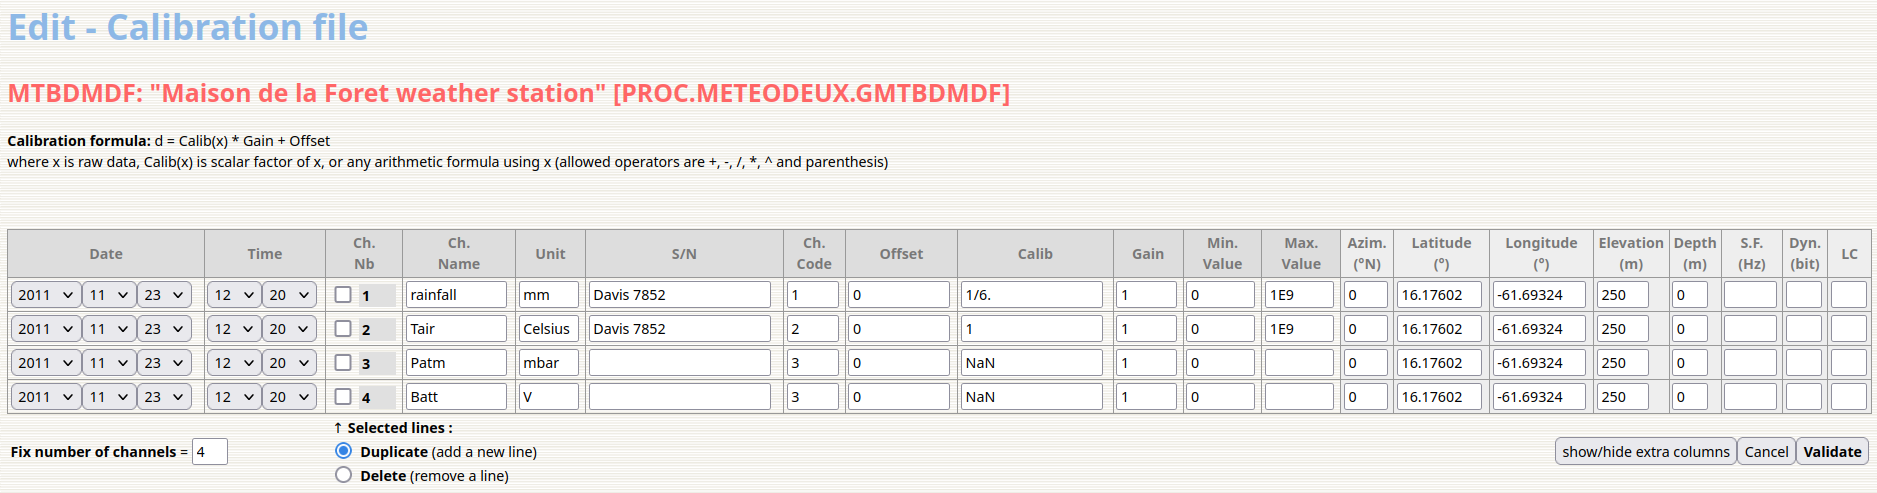
\includegraphics[width=\textwidth]{figures/theia/calib_file_form.png}
	\caption{Calibration file editor}
	\label{formCLB}
\end{figure}

